\subsection{The Haynes \& Shockley experiment}
\subsubsection{Measuring at constant $U$}
In this first part, we measured the response in the germanium block to 
the laser pulse at constant voltage $U = (49.6 \pm 0.8)\,$V, 
changing the distance between the point where the laser enters 
and the needle $d$ over a range from 1 to 10 mm. 

Taking the measurements, we had to cope with various difficulties. 
Most notably, the observability of even the signal 
of the laser itself ceased at one point, probably due to the needle 
loosing contact or other technical issues. 
After trying to readjust the setup, we did observe a signal 
again. 
Only doing the evaluation did we notice that this also resulted in 
a large offset in time for all following measurements. 
Thus, the first four measurements have to be ignored. The offset 
remained stable for all but one ('File 7') of the further measurements. 
Furthermore, another set was so badly influenced by noise that 
a gaussian fit has no chance to converge. 
For the remaining data, we apply the following scheme: 
In order to facilitate the convergence of the fitting algorithm, 
we took the according set of smooth data, which is simply the 
average of 128 measurements done by the oscilloscope. 
The resulting parameters are then passed to the algorithm
as initial guesses for a fit on the original data. 
This is shown for an exemplary case in figure \ref{fig:h_s_raw_28}, 
where the measured distance $d$ has been measured to 
$d = 3.7 \pm 0.5\,$mm. 
The parameters obtained by the fit with the original data 
are shown in a box within the plot as well. 
The fitted offset is omitted as it will not be used in any further 
calculation. The errors 
are obtained by the fitting algorithm as the square root of the 
diagonal entries. We did not further add an error on the 
$U$-value, as the scattering should be indication of 
uncertainty enough. For the oscilloscope, only 
a DC vertical accuracy is stated which would 
only apply for the offset. 
In the further calculations, we ignore the 
off-diagonal elements since the desired quantities each depend 
on only one parameter. 
\begin{figure}
    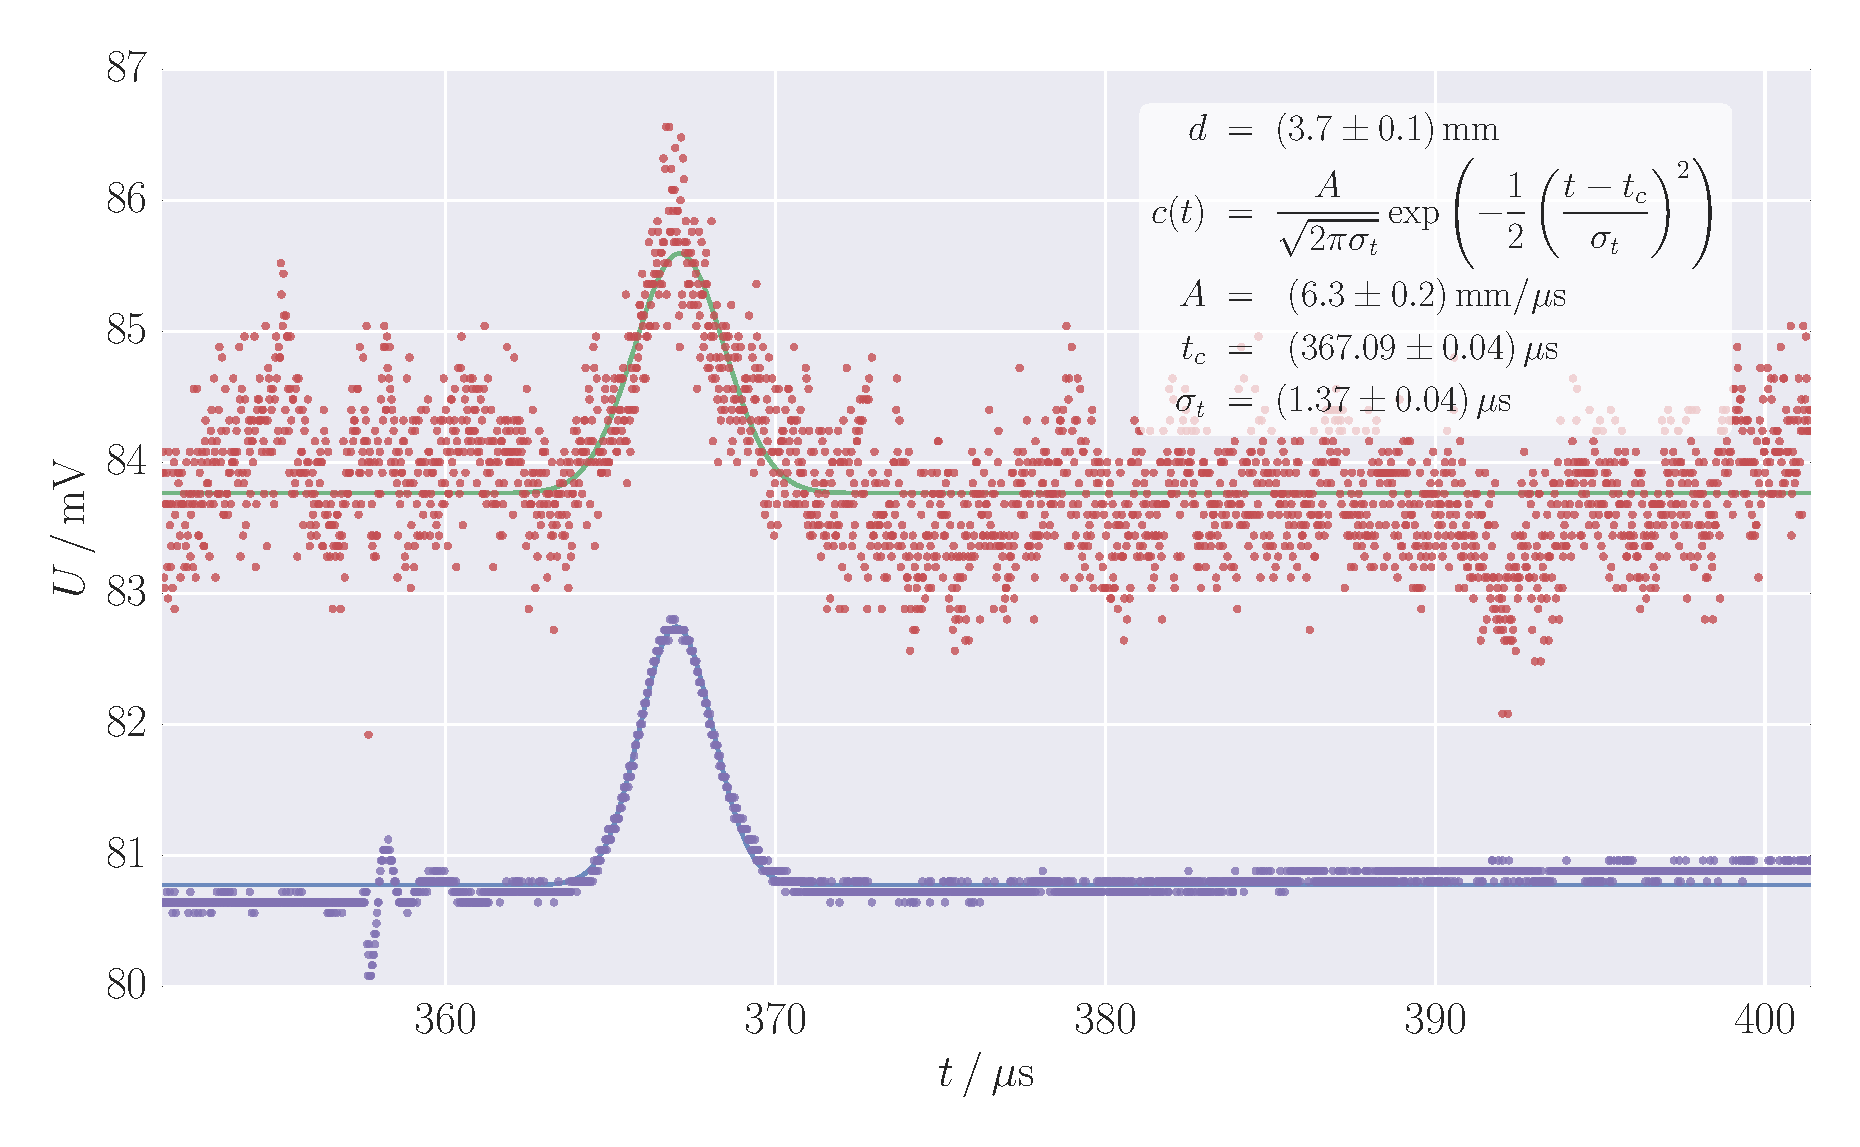
\includegraphics[width=1.0\textwidth]{figures/haynes_shockley_raw_28}
    \caption{
        Raw data and fitted gaussians for $d = 3.7 \pm 0.5\,$cm. 
        The lower, much more scattered data is taken without averaging 
        while the upper corresponds to the average of 128 measurements, where the 
        running average is done by the oscilloscope directly. This smoother data is 
        used to obtain the guesses for the fit on the noisy data, 
        while all further calculations are done with the original, 
        non-averaged data. 
        One can observe the large offset which is of unknown origin appearing 
        after a temporary loss of signal and small adjustments on the setup.
        }
    \label{fig:h_s_raw_28}
\end{figure}

Plots of all used data (original and smooth ones) with the 
fitted functions drawn are shown in the appendix, 
see~\ref{sec:appendix_h_s_plots}.
For all further calculations, the smoothed data is ignored 
and each calculation is done with the non-averaged ones. 
Errors will always be taken to be those of the fits.
An overview of the fitted parameters at corresponding 
distance $d$ is given in table~\ref{tab:h_s_fit_parameters}.
\renewcommand{\arraystretch}{1.5}
\begin{table}[htdp]
    \centering
    \caption{
        Results of fits with gaussians for all used data sets with distance 
        $d$ between laser and needle. The $\chi^2$-tests are quite high due to the 
        noise and tendencies to ascend on the scale of 10 sigma (compare figures, 
        e.~g.smooth data in figure~\ref{fig:h_s_raw_28}).
        }
    	\begin{tabular}{|p{2cm}|p{3cm}|p{3cm}|p{3cm}|p{2cm}|}
		\hline
		\rowcolor{tabcolor}
		$d \, / \, \mathrm{mm}$        & $A \, / \, \mathrm{\frac{mm}{\mu s}})$ & 
 			$t_c \, / \, \mathrm{\mu s}$    & $\sigma_t \, / \, \mathrm{\mu s}$ & 
 			$\chi^2 / n_d$ \\ \hline
		$7.5$ & $3.2 \pm 0.2$ & $377.54 \pm 0.13$ & $1.93 \pm 0.13$ & $10.2$\\ 
		$8.5$ & $3.3 \pm 0.3$ & $378.28 \pm 0.20$ & $1.98 \pm 0.20$ & $3.0$\\ 
		$8.0$ & $2.5 \pm 0.3$ & $377.58 \pm 0.20$ & $1.69 \pm 0.20$ & $2.8$\\ 
		$7.5$ & $2.7 \pm 0.2$ & $376.50 \pm 0.11$ & $1.23 \pm 0.11$ & $2.6$\\ 
		$5.9$ & $3.0 \pm 0.2$ & $372.45 \pm 0.09$ & $1.05 \pm 0.09$ & $3.4$\\ 
		$4.4$ & $4.0 \pm 0.2$ & $368.91 \pm 0.05$ & $1.14 \pm 0.05$ & $9.9$\\ 
		$3.9$ & $3.8 \pm 0.2$ & $367.71 \pm 0.05$ & $1.12 \pm 0.05$ & $12.3$\\ 
		$3.7$ & $6.3 \pm 0.2$ & $367.09 \pm 0.04$ & $1.37 \pm 0.04$ & $12.3$\\ 
		$1.1$ & $12.2 \pm 0.2$ & $362.66 \pm 0.01$ & $0.95 \pm 0.01$ & $12.3$\\ 
		\hline
	\end{tabular}

    \label{tab:h_s_fit_parameters}
\end{table}

The obtained center of the gaussians $t_c$ are plotted over the 
according distances. With a linear fit, we calculate $\mu_n E$. 
The results are shown in figure~\ref{fig:h_s_mu_e_d}. 
With the length $l = (3.0 \pm 0.5)\,$mm for the germanium strip and 
applied voltage $U = (49.6 \pm 0.8)\,$V we calculate an electric field of 
\begin{equation}
    E = \frac{U}{d} = (1.65 \pm 0.04)\, \mathrm{\frac{V}{mm}}\, .
\end{equation}
The electron mobility is then calculated to 
\begin{equation}
    \begin{split}
        \mu_n   &= (0.264 \pm 0.013)\, \mathrm{\frac{mm^2}{V\mu s}} \\
                &= (2640 \pm 130)\, \mathrm{\frac{cm^2}{V\,s}} \,.
    \end{split}
\end{equation}
Although the literature value~\cite{staatsexamen} of 
\begin{equation}
    \mu_{n, \mathrm{lit}} = 3900\, \mathrm{\frac{cm^2}{V\,s}}
\end{equation}
is far off the measured value (by 10 standard deviations --  showing the 
    enormous underestimation of systematical errors applying purely 
    intrinsic estimation and propagation), the calculated value 
does agree in magnitude. It is further expected that the physical 
reality under consideration, namely the electrons moving close to the surface 
of the sample, does change all parameters considerably. 


\begin{figure}
    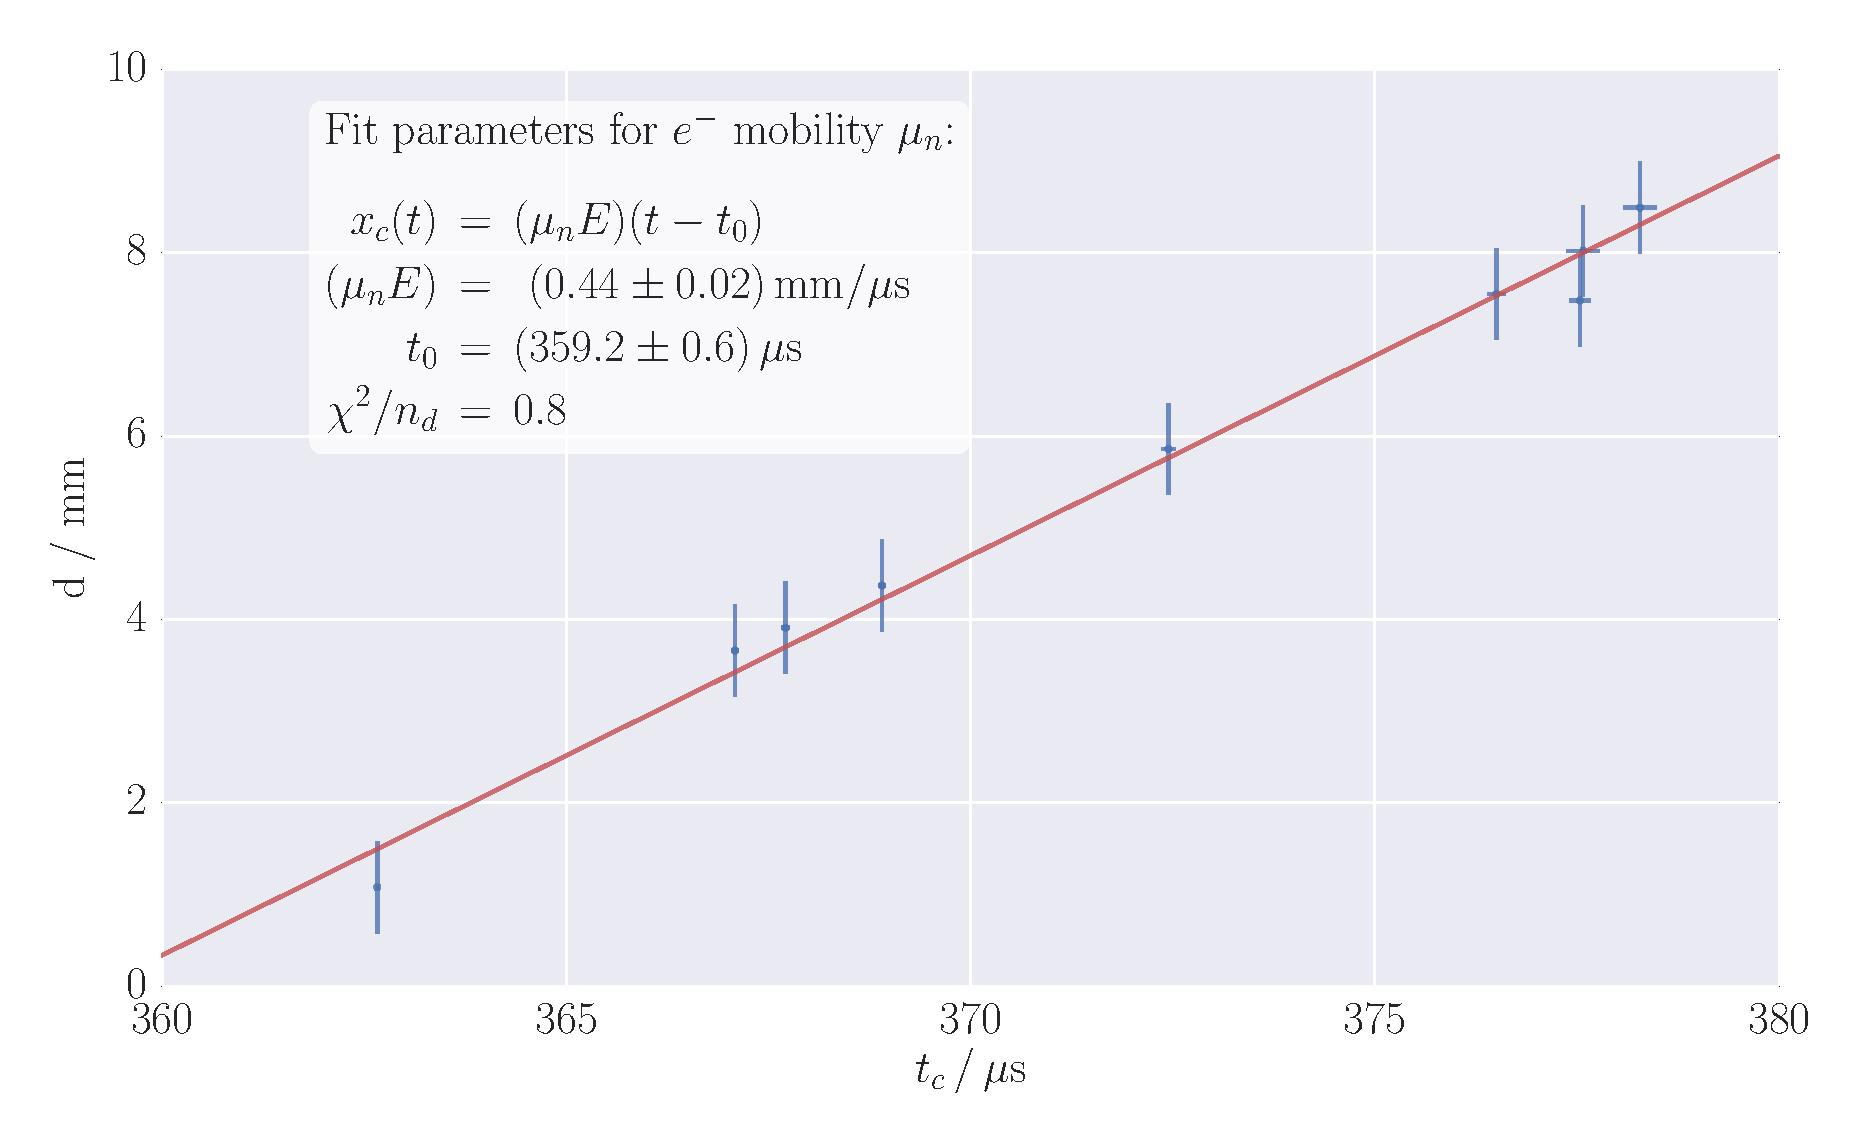
\includegraphics[width=1.0\textwidth]{figures/haynes_shockley_mu_e_d}
    \caption{
        Fitted straight line on centers of gaussians as calculated before. 
        The linear behavior is see quite well, as indicated also by the 
        $\chi^2$-test.
        }
    \label{fig:h_s_mu_e_d}
\end{figure}

With the velocity $v = \mu_n E$ calculated, we can transform 
the temporal sigma to a spatial one as described in the procedure section~%
\ref{sec:transform_x_t}. We can then perform the exponential fit on 
the amplitudes $A(t_c)$ at the maximum, as shown in figure~\ref{fig:h_s_tau_d}.
Here, the fit does not yield such a good result. The errors obtained 
by the gaussian fits seem to underestimate the real uncertainty 
which might be subject to several systematic errors, as will be described later on. 
The life time $\tau_n$ of the electrons is a yielded directly by the fit:
\begin{equation}
    \tau_n = (6.7 \pm 1.0)\, \mathrm{\mu s} \, .
\end{equation}
The literature value $\tau_{n, \mathrm{lit}} = (45 \pm 2)\, \mathrm{\mu s}$%
~\cite{staatsexamen}
is one magnitude above our results. Aside the systematical errors already 
mentioned, the measured value corresponds to a somewhat different 
physical reality: As the laser only enters the first $0.5 \, \mathrm{\mu m}$
of the sample~\cite{staatsexamen}, we expect the lattice defects to have 
a large effect especially on the recombination rate. Theoretically, 
these effects are much harder to calculate -- experimentally, however, 
it turns out that the defects drastically reduce the life time of free electrons. 

\begin{figure}
    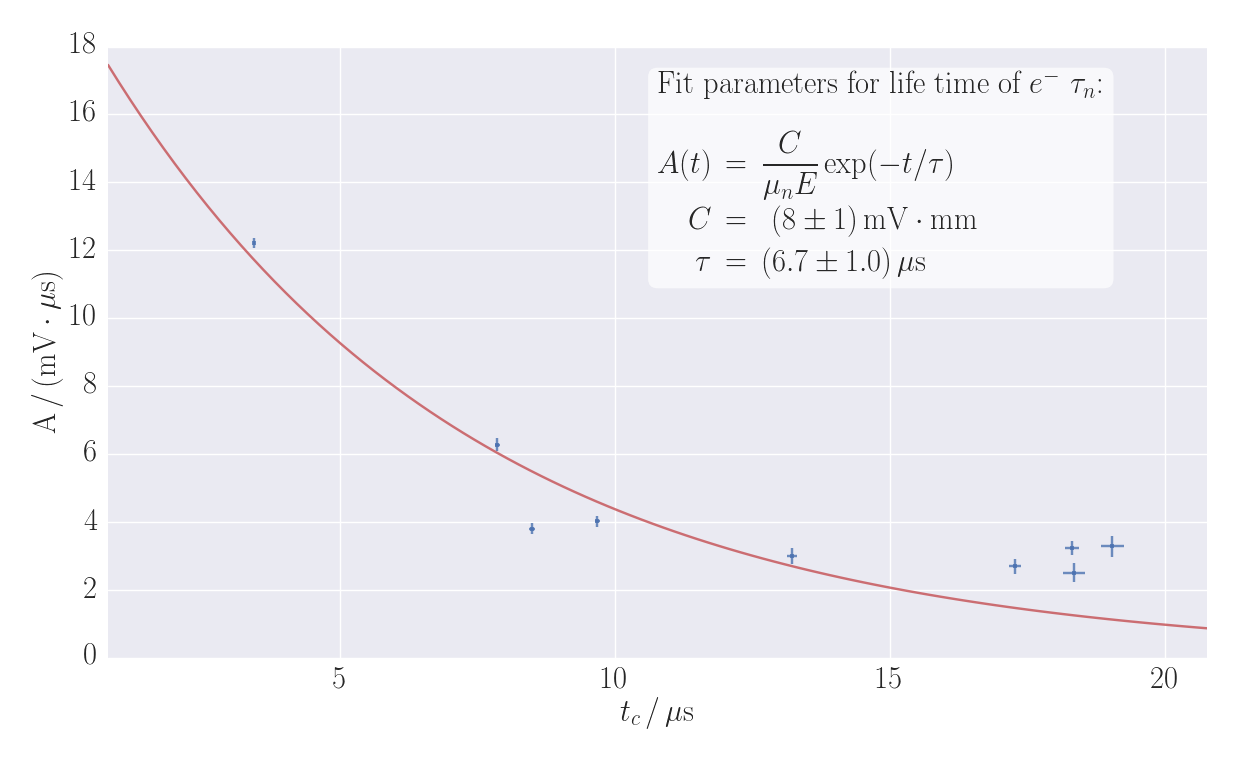
\includegraphics[width=1.0\textwidth]{figures/haynes_shockley_tau_d}
    \caption{
        Exponential fit through the amplitudes obtained by the gaussian fits 
        in order to calculated the electron life time $\tau$. The $\chi^2$-test 
        as well as the graphical impression shows that the errors obtained by the 
        linear regression do not mirror the fluctuations obtained. It could 
        further be the case that systematical errors have a large impact on the 
        data. 
        }
    \label{fig:h_s_tau_d}
\end{figure}

In the ultimate part of evaluating this measurement, the standard deviations in 
time $\sigma_t$ are transferred to those in space $\sigma_x$ as described before. 
The spatial variances $\sigma_x^2$ are then fitted linearly over the time 
traveled by the electrons $t_c$. The result is shown in figure~\ref{fig:h_s_D_d}.
Even more so then in the prior fit the data does not show the expected behavior 
but instead fluctuates widely due to the systematical errors and noise. 
The obtained value of electron diffusion constant 
\begin{equation}
    D_n = (140 \pm 20)\, \mathrm{\frac{cm^2}{s}} 
\end{equation}
can thus be regarded only as an assessor of the magnitude of the real $D_n$ 
of electrons in germanium. The comparison with the literature value~\cite{staatsexamen}, 
\begin{equation}
    D_{n, \mathrm{lit}} = 101\, \mathrm{\frac{cm^2}{s}}
\end{equation}
shows the agreement in magnitude. The difference of two sigma again shows the 
underestimation of errors by mere propagation. 

\begin{figure}
    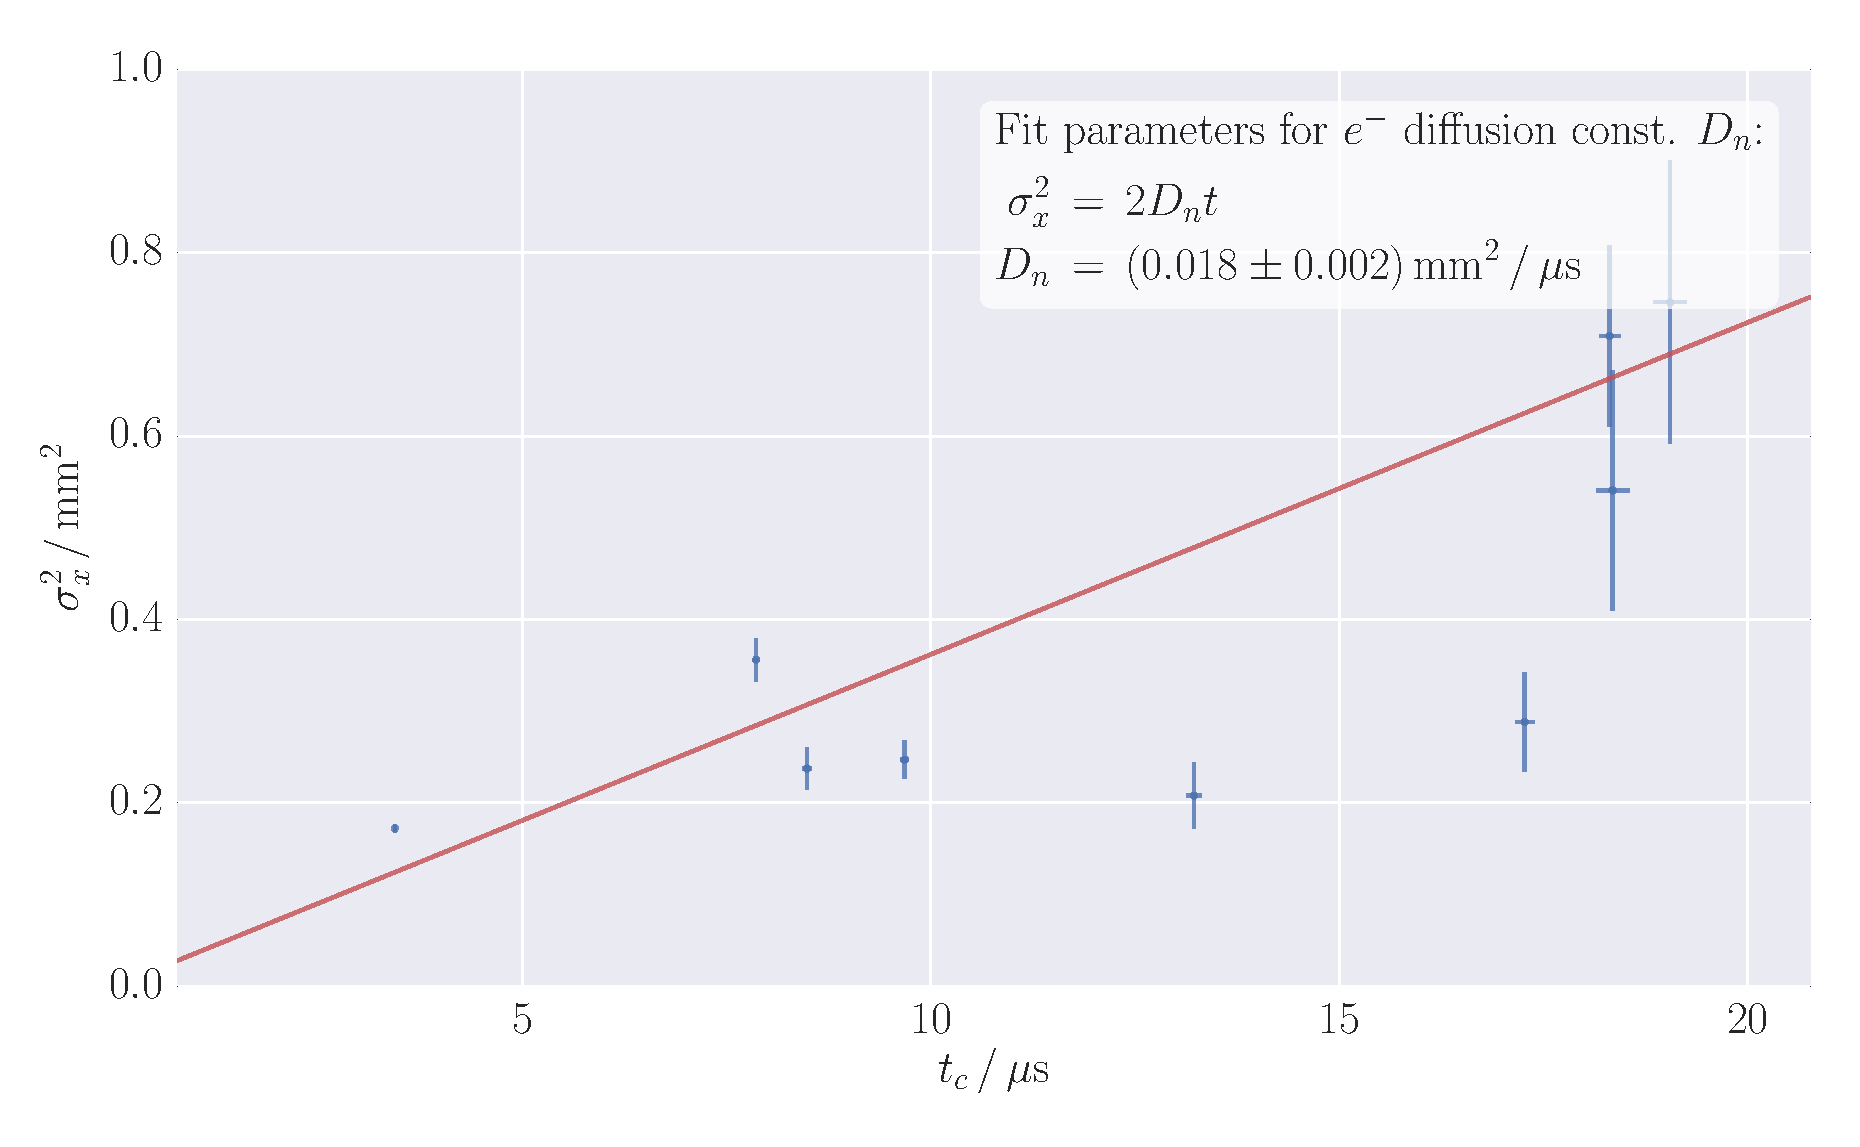
\includegraphics[width=1.0\textwidth]{figures/haynes_shockley_D_d}
    \caption{
        Spatial variances $\sigma_x^2$ fitted over center of gaussians $t_c$ 
        (corresponding to the time traveled by the distribution) with a linear 
        function in order to calculate the diffusion constant $D_n$ of electrons. 
        One clearly observes the strong disagreement of the obtained data and the 
        expectation. We refer to multiple sources of systematic errors and fluctuations 
        explaining this contrast. 
        }
    \label{fig:h_s_D_d}
\end{figure}
\FloatBarrier

\subsubsection{Measuring at constant $U$}
The procedure of this part of the experiment is roughly the same as before. 
Instead of changing the distance, we change the applied acceleration voltage 
$U_mathrm{acc}$, while $d$ remains constant at $d = (4.1 \pm 0.5)\,$mm. 
The raw data and fitted gaussians are all displayed in the appendix,
\ref{sec:appendix_h_s_plots_U}. A summary of the calculated parameters is 
again given in a table (\ref{tab:h_s_fit_parameters_U}). 
\renewcommand{\arraystretch}{1.5}
\begin{table}[htdp]
    \centering
    \caption{
        Results of fits with gaussians for all used data sets with variating 
        acceleration voltage
        $U_\mathrm{acc}$. Again, the $\chi^2$-tests are quite high due to 
        large scale fluctuations and noise. 
        }
    	\begin{tabular}{|p{2cm}|p{3cm}|p{3cm}|p{3cm}|p{2cm}|}
		\hline
		\rowcolor{tabcolor}
		$U_\mathrm{acc} \, / \, \mathrm{V}$        & $A \, / \, \mathrm{\frac{mm}{\mu s}}$ & 
     			$t_c \, / \, \mathrm{\mu s}$    & $\sigma_t \, / \, \mathrm{\mu s}$ & 
     			$\chi^2 / n_d$ \\ \hline
		$24.4$ & $2.6 \pm 0.3$ & $371.66 \pm 0.20$ & $1.82 \pm 0.20$ & $2.3$\\ 
		$32.8$ & $3.8 \pm 0.1$ & $368.12 \pm 0.04$ & $1.09 \pm 0.04$ & $9.0$\\ 
		$39.6$ & $2.4 \pm 0.2$ & $370.18 \pm 0.16$ & $1.50 \pm 0.16$ & $2.4$\\ 
		$41.2$ & $7.9 \pm 0.2$ & $366.72 \pm 0.03$ & $1.15 \pm 0.03$ & $115.0$\\ 
		$44.4$ & $8.0 \pm 0.3$ & $367.85 \pm 0.07$ & $1.55 \pm 0.08$ & $5.1$\\ 
		$46.4$ & $3.5 \pm 0.1$ & $368.25 \pm 0.04$ & $0.99 \pm 0.04$ & $9.1$\\ 
		$48.0$ & $4.3 \pm 0.2$ & $367.52 \pm 0.05$ & $1.08 \pm 0.05$ & $14.6$\\ 
		$48.4$ & $7.4 \pm 0.2$ & $366.68 \pm 0.03$ & $1.29 \pm 0.03$ & $10.3$\\ 
		$49.6$ & $7.3 \pm 0.1$ & $367.20 \pm 0.02$ & $1.40 \pm 0.03$ & $39.0$\\ 
		\hline
	\end{tabular}

    \label{tab:h_s_fit_parameters_U}
\end{table}

All fitted gaussians are displayed in figure%
~\ref{fig:h_s_all_gauss_U}. The expected distribution of descending amplitudes 
and enlarging widths is only partially observed -- a fact that will impede the 
further analysis. 
\begin{figure}
    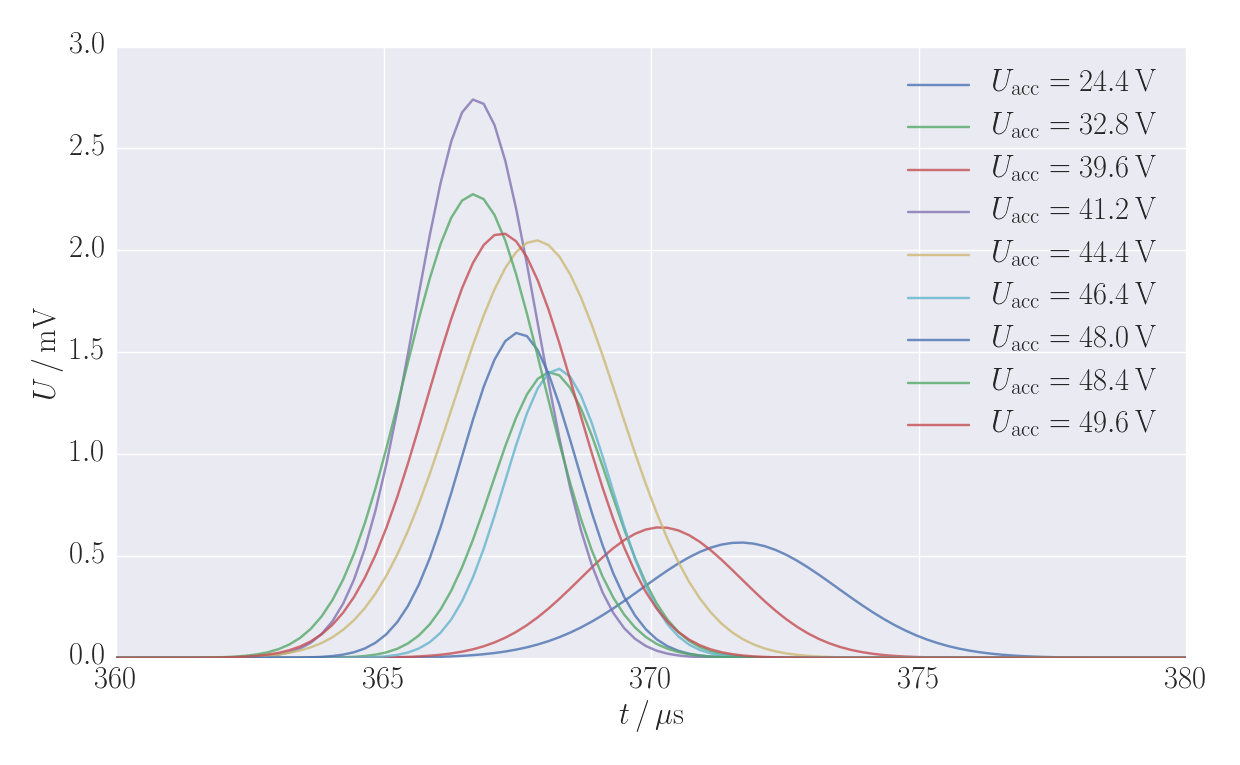
\includegraphics[width=1.0\textwidth]{figures/haynes_shockley_all_gauss_U}
    \caption{
        Fitted gaussian for constant $d$, variating the acceleration voltage 
        $U_\mathrm{acc}$. From the theory, one would expect the amplitudes to decline with 
        time $t$, while the distribution would get wider. This feature is only 
        partially given in our data. 
        }
    \label{fig:h_s_all_gauss_U}
\end{figure}
In order to get the linear correspondence between temporal and 
spatial center of the distribution, $t_c$ and $x_c$, we 
exchange one term of the defining equation \eqref{eq:x_c} and get 
\begin{equation}
    \frac{x_c}{E} = \mu_n t \, .
\end{equation}
With $x_c = d$ and $E = U_\mathrm{acc} / l$, we apply a fit of the form
\begin{equation}
    \frac{d \, l}{U_\mathrm{acc}} = \mu_n (t - t_0) \, ,
\end{equation}
where $t_0$ refers to the offset in time we observed. The result 
is shown in figure~\ref{fig:h_s_mu_e_U}. Although the fit is clearly underfed, 
as fluctuations of the observable magnitude would require a much larger 
set of data, we continue the calculation with the obtained parameters. 
Here, the electron mobility is directly calculated with 
\begin{equation}
    \begin{split}
        \mu_e   = (0.30 \pm 0.12)\, \mathrm{\frac{mm^2}{V\mu s}} \\
                = (3000 \pm 120)\, \mathrm{\frac{cm^2}{V\,s}} \,.
    \end{split}
\end{equation}
The value again lies notably below the accepted value. It does agree 
with the value measured in the first experiment within three standard deviations, 
which at least indicates the consistency of the results. 
\begin{figure}
    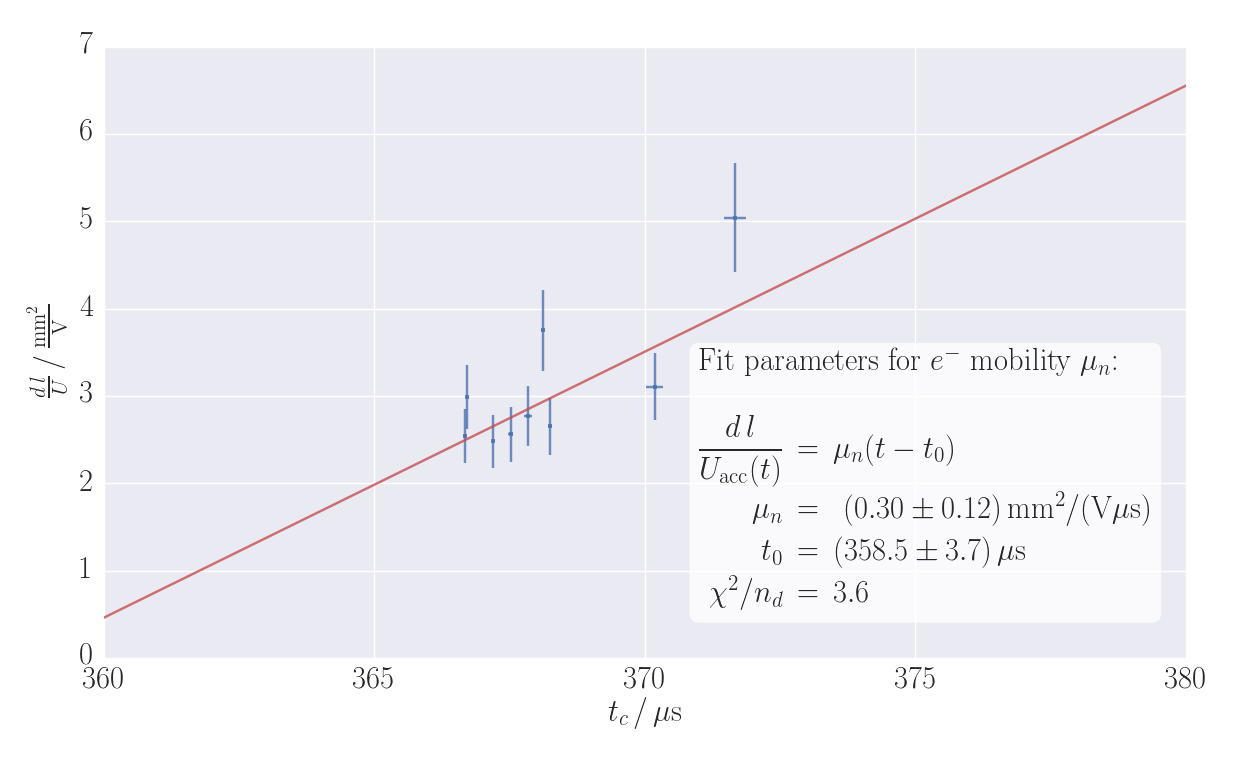
\includegraphics[width=1.0\textwidth]{figures/haynes_shockley_mu_e_U}
    \caption{
        Fitted straight line on centers of gaussians for constant $d$.  
        The little number of data points does not allow for a good fit. 
        Further, the errors obtained from fitting the gaussians do not
        capture the real errors, which might further be due to 
        fluctuations. This is also indicated by the $\chi^2$-test.
        }
    \label{fig:h_s_mu_e_d}
\end{figure}
We continue calculating the life time $\tau_n$, applying the 
transformation of the amplitude $C' = C / (\mu_n E)$. The resulting 
parameters together with the fit on the obtained data points is shown 
in figure~\ref{fig:h_s_tau_U}, yielding a life time of 
\begin{equation}
    \tau_n = (1.6 \pm 0.5)\, \mathrm{\mu s} \, .
\end{equation}
This parameter is in the same order of magnitude as the one obtained 
by the first measurement, but smaller and thus ever further away from 
the literature value. The discussion done before applies here as well. 
\begin{figure}
    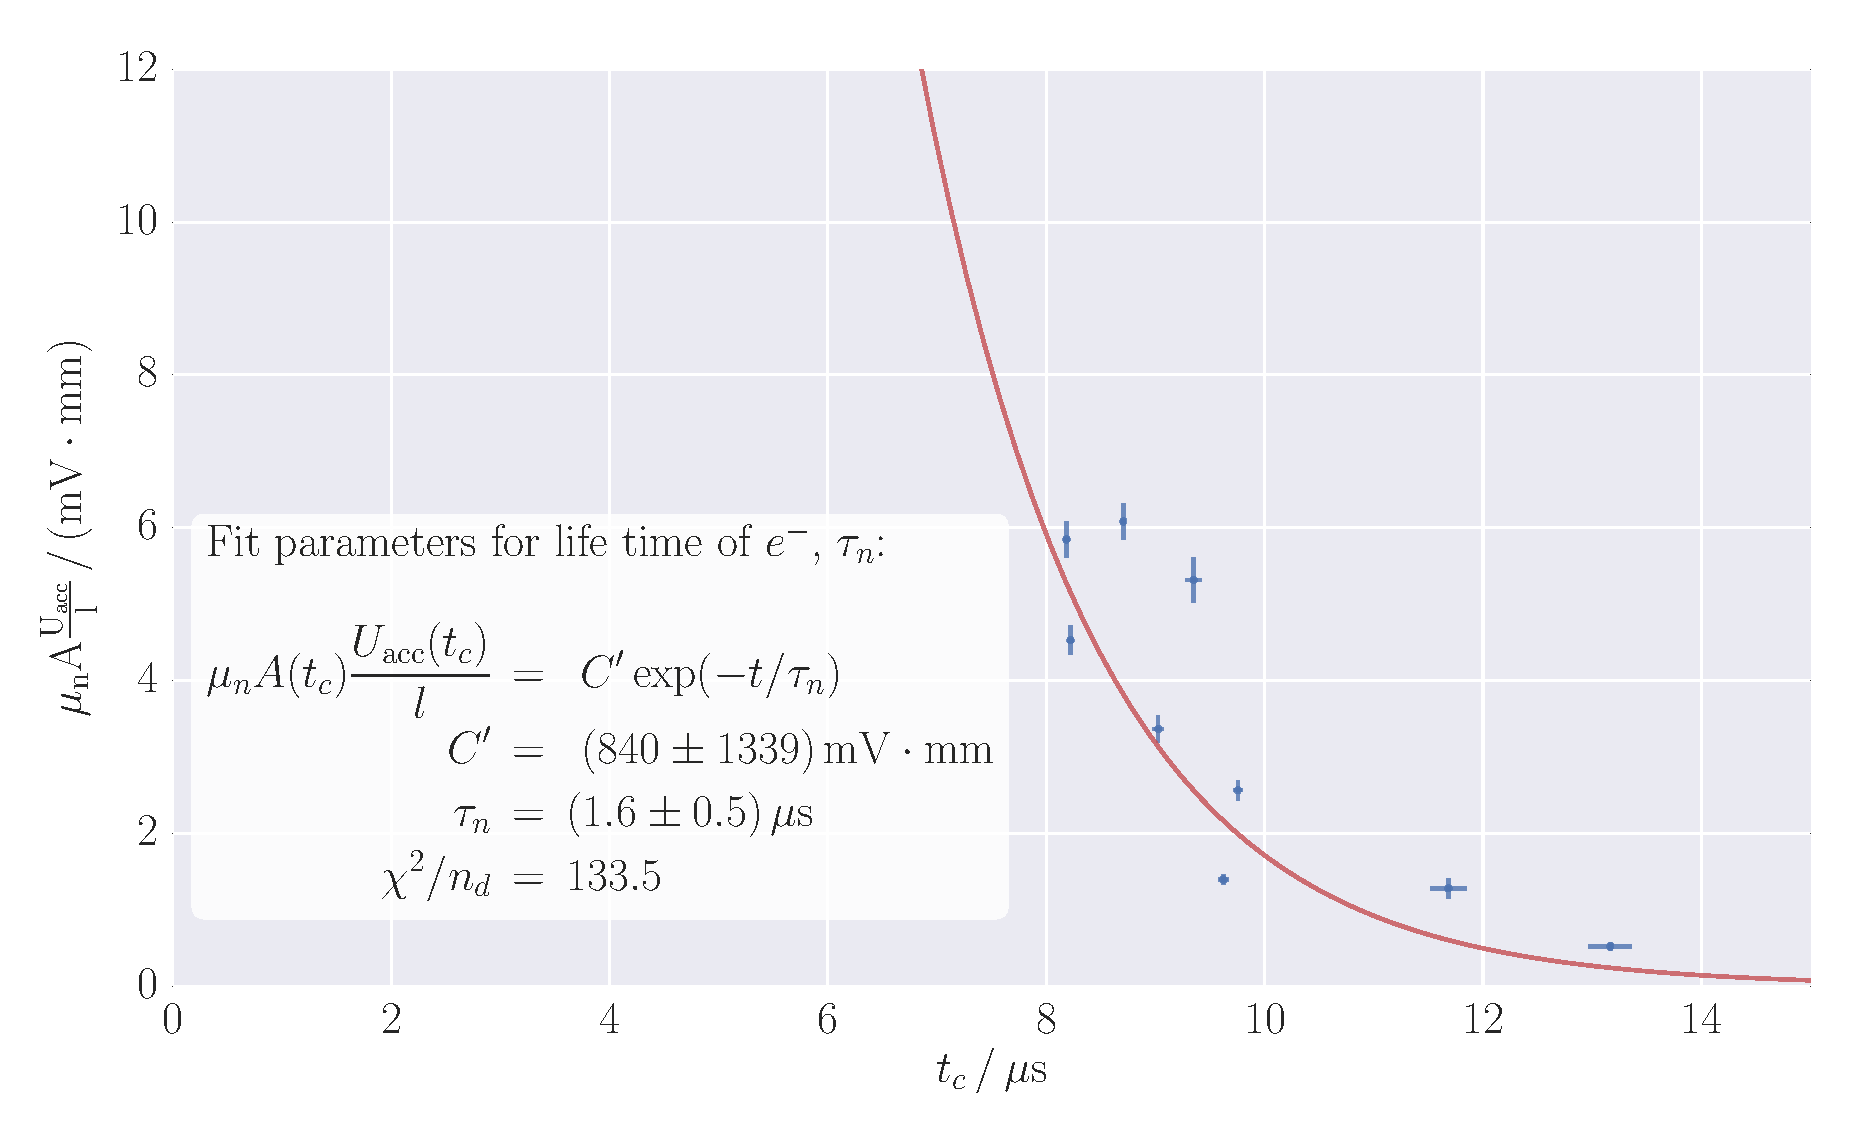
\includegraphics[width=1.0\textwidth]{figures/haynes_shockley_tau_U}
    \caption{
        Exponential fit to calculate the life time of free electrons in germanium. 
        The errors, stemming from the fit of gaussians on the original data, 
        are much to small, since they do not capture global fluctuations induced 
        by systematic errors. The resulting physical parameter $\tau_n$ should 
        thus be interpreted with care, using it as an approximation of the 
        order of magnitude. 
        }
    \label{fig:h_s_tau_U}
\end{figure}
The third and last calculation of this part of the experiment is the fit over the 
variances which are obtained analogously to the ones before by applying the 
described transformation from temporal to spatial quantities. 
In this case, however, the electron velocity is dependent on 
the voltage, yielding a different transformation for each $\sigma_t$. 
We will not further show intermediate steps of the transformations and 
plot only the resulting data with fits, see figure~\ref{fig:h_s_D_U}. 
The resulting fitted parameter of 
\begin{equation}
    D_n = (130 \pm 20)\, \mathrm{\frac{cm^2}{s}} 
\end{equation}
resembles the one measured before quite well. Considering the 
strong variance and low quality of the fit, this rather seems to 
be coincidental and should by no means obscure the large uncertainty 
and underestimation of the error due to systematical errors. 
\begin{figure}
    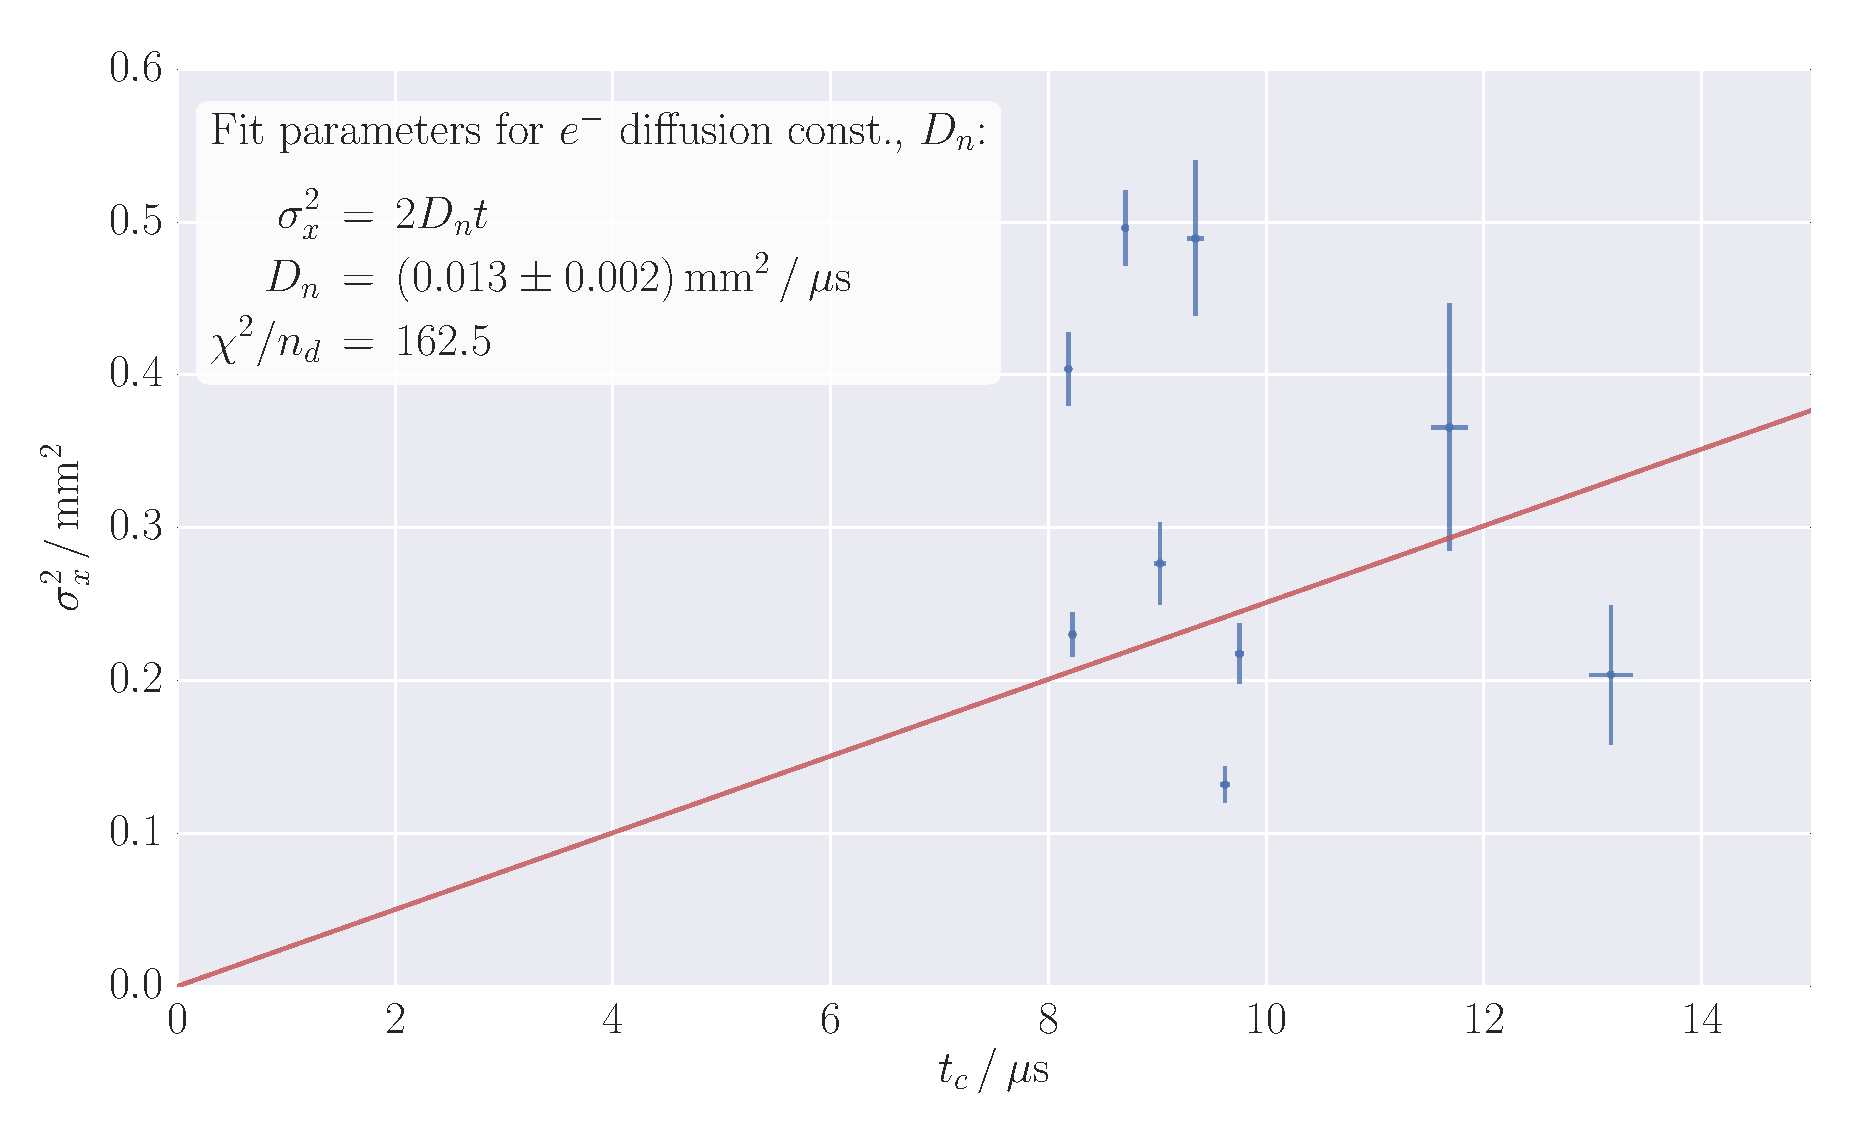
\includegraphics[width=1.0\textwidth]{figures/haynes_shockley_D_U}
    \caption{
        Linear fit through spatial variances $\sigma_x^2$. 
        The data does not seem to follow a linear behavior. 
        The usability of the result to assess the order of magnitude 
        of $D_n$ stems from the constraint of $\sigma_x^2(t = 0) = 0$, 
        has to be used very conservatively, though. The error 
        is only realistic if the constraint is taken as fixed -- 
        a non-zero variance for $t = 0$ would allow a much wider range of
        linear fits and thus a much higher uncertainty. 
        }
    \label{fig:h_s_D_U}
\end{figure}


